\begin{figure}[!htbp]
\centering
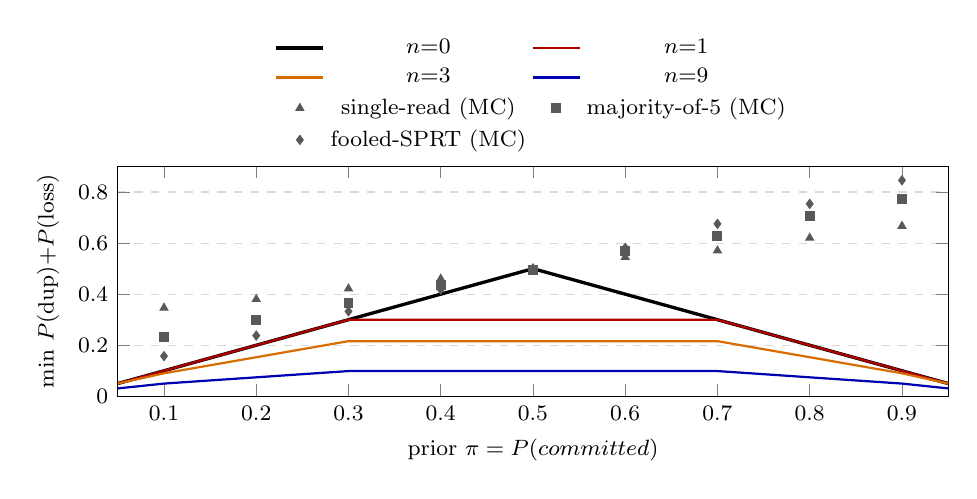
\begin{tikzpicture}
\begin{axis}[width=\linewidth,height=4.5cm,xlabel={prior $\pi=P(\text{committed})$},ylabel={min $P(\mathrm{dup}){+}P(\mathrm{loss})$},
  ymin=0,ymax=0.9,xmin=0.05,xmax=0.95,legend columns=2,
  legend style={at={(0.5,1.02)},anchor=south,font=\footnotesize,draw=none,fill=none},
  ymajorgrids,grid style={dashed,gray!30},tick label style={font=\footnotesize},label style={font=\footnotesize}]
\addplot[color=black,very thick] coordinates {(0.05,0.0500) (0.10,0.1000) (0.15,0.1500) (0.20,0.2000) (0.25,0.2500) (0.30,0.3000) (0.35,0.3500) (0.40,0.4000) (0.45,0.4500) (0.50,0.5000) (0.55,0.4500) (0.60,0.4000) (0.65,0.3500) (0.70,0.3000) (0.75,0.2500) (0.80,0.2000) (0.85,0.1500) (0.90,0.1000) (0.95,0.0500)};
\addlegendentry{$n{=}0$}
\addplot[color=red!70!black,thick] coordinates {(0.05,0.0500) (0.10,0.1000) (0.15,0.1500) (0.20,0.2000) (0.25,0.2500) (0.30,0.3000) (0.35,0.3000) (0.40,0.3000) (0.45,0.3000) (0.50,0.3000) (0.55,0.3000) (0.60,0.3000) (0.65,0.3000) (0.70,0.3000) (0.75,0.2500) (0.80,0.2000) (0.85,0.1500) (0.90,0.1000) (0.95,0.0500)};
\addlegendentry{$n{=}1$}
\addplot[color=orange!85!black,thick] coordinates {(0.05,0.0500) (0.10,0.0900) (0.15,0.1215) (0.20,0.1530) (0.25,0.1845) (0.30,0.2160) (0.35,0.2160) (0.40,0.2160) (0.45,0.2160) (0.50,0.2160) (0.55,0.2160) (0.60,0.2160) (0.65,0.2160) (0.70,0.2160) (0.75,0.1845) (0.80,0.1530) (0.85,0.1215) (0.90,0.0900) (0.95,0.0500)};
\addlegendentry{$n{=}3$}
\addplot[color=blue!70!black,thick] coordinates {(0.05,0.0309) (0.10,0.0498) (0.15,0.0621) (0.20,0.0743) (0.25,0.0866) (0.30,0.0988) (0.35,0.0988) (0.40,0.0988) (0.45,0.0988) (0.50,0.0988) (0.55,0.0988) (0.60,0.0988) (0.65,0.0988) (0.70,0.0988) (0.75,0.0866) (0.80,0.0743) (0.85,0.0621) (0.90,0.0498) (0.95,0.0309)};
\addlegendentry{$n{=}9$}
\addplot[only marks,mark=triangle*,mark size=1.6pt,gray!70!black] coordinates {(0.10,0.3462) (0.20,0.3804) (0.30,0.4217) (0.40,0.4600) (0.50,0.4982) (0.60,0.5452) (0.70,0.5706) (0.80,0.6202) (0.90,0.6668)};
\addlegendentry{single-read (MC)}
\addplot[only marks,mark=square*,mark size=1.6pt,gray!70!black] coordinates {(0.10,0.2336) (0.20,0.2999) (0.30,0.3656) (0.40,0.4355) (0.50,0.4951) (0.60,0.5691) (0.70,0.6267) (0.80,0.7063) (0.90,0.7709)};
\addlegendentry{majority-of-5 (MC)}
\addplot[only marks,mark=diamond*,mark size=1.6pt,gray!70!black] coordinates {(0.10,0.1573) (0.20,0.2379) (0.30,0.3327) (0.40,0.4179) (0.50,0.5008) (0.60,0.5814) (0.70,0.6753) (0.80,0.7537) (0.90,0.8462)};
\addlegendentry{fooled-SPRT (MC)}
\end{axis}
\end{tikzpicture}
\caption{Sanity check of Theorem~\ref{thm:main}(d). Lines: exact Bayes floor $\mathbb{E}[\min(\pi_n,1{-}\pi_n)]$ after $n$ reads of an
informative probe ($\epsilon{=}0.3$). Markers: policies against an \emph{uninformative} probe (20{,}000 episodes each); none goes below $n{=}0$.}
\label{fig:floor}
\end{figure}
